\PassOptionsToPackage{unicode=true}{hyperref} % options for packages loaded elsewhere
\PassOptionsToPackage{hyphens}{url}
%
\documentclass[ignorenonframetext,]{beamer}
\usepackage{pgfpages}
\setbeamertemplate{caption}[numbered]
\setbeamertemplate{caption label separator}{: }
\setbeamercolor{caption name}{fg=normal text.fg}
\beamertemplatenavigationsymbolsempty
% Prevent slide breaks in the middle of a paragraph:
\widowpenalties 1 10000
\raggedbottom
\setbeamertemplate{part page}{
\centering
\begin{beamercolorbox}[sep=16pt,center]{part title}
  \usebeamerfont{part title}\insertpart\par
\end{beamercolorbox}
}
\setbeamertemplate{section page}{
\centering
\begin{beamercolorbox}[sep=12pt,center]{part title}
  \usebeamerfont{section title}\insertsection\par
\end{beamercolorbox}
}
\setbeamertemplate{subsection page}{
\centering
\begin{beamercolorbox}[sep=8pt,center]{part title}
  \usebeamerfont{subsection title}\insertsubsection\par
\end{beamercolorbox}
}
\AtBeginPart{
  \frame{\partpage}
}
\AtBeginSection{
  \ifbibliography
  \else
    \frame{\sectionpage}
  \fi
}
\AtBeginSubsection{
  \frame{\subsectionpage}
}
\usepackage{lmodern}
\usepackage{amssymb,amsmath}
\usepackage{ifxetex,ifluatex}
\usepackage{fixltx2e} % provides \textsubscript
\ifnum 0\ifxetex 1\fi\ifluatex 1\fi=0 % if pdftex
  \usepackage[T1]{fontenc}
  \usepackage[utf8]{inputenc}
  \usepackage{textcomp} % provides euro and other symbols
\else % if luatex or xelatex
  \usepackage{unicode-math}
  \defaultfontfeatures{Ligatures=TeX,Scale=MatchLowercase}
\fi
% use upquote if available, for straight quotes in verbatim environments
\IfFileExists{upquote.sty}{\usepackage{upquote}}{}
% use microtype if available
\IfFileExists{microtype.sty}{%
\usepackage[]{microtype}
\UseMicrotypeSet[protrusion]{basicmath} % disable protrusion for tt fonts
}{}
\IfFileExists{parskip.sty}{%
\usepackage{parskip}
}{% else
\setlength{\parindent}{0pt}
\setlength{\parskip}{6pt plus 2pt minus 1pt}
}
\usepackage{hyperref}
\hypersetup{
            pdftitle={Markets and Models},
            pdfauthor={Kiernan Nicholls},
            pdfborder={0 0 0},
            breaklinks=true}
\urlstyle{same}  % don't use monospace font for urls
\newif\ifbibliography
\usepackage{longtable,booktabs}
\usepackage{caption}
% These lines are needed to make table captions work with longtable:
\makeatletter
\def\fnum@table{\tablename~\thetable}
\makeatother
\usepackage{graphicx,grffile}
\makeatletter
\def\maxwidth{\ifdim\Gin@nat@width>\linewidth\linewidth\else\Gin@nat@width\fi}
\def\maxheight{\ifdim\Gin@nat@height>\textheight\textheight\else\Gin@nat@height\fi}
\makeatother
% Scale images if necessary, so that they will not overflow the page
% margins by default, and it is still possible to overwrite the defaults
% using explicit options in \includegraphics[width, height, ...]{}
\setkeys{Gin}{width=\maxwidth,height=\maxheight,keepaspectratio}
\setlength{\emergencystretch}{3em}  % prevent overfull lines
\providecommand{\tightlist}{%
  \setlength{\itemsep}{0pt}\setlength{\parskip}{0pt}}
\setcounter{secnumdepth}{0}

% set default figure placement to htbp
\makeatletter
\def\fps@figure{htbp}
\makeatother


\title{Markets and Models}
\author{Kiernan Nicholls}
\date{Spring, 2019}

\begin{document}
\frame{\titlepage}

\begin{frame}{Why predict elections?}
\protect\hypertarget{why-predict-elections}{}

\begin{itemize}
\tightlist
\item
  Resource allocation
\item
  Strategy adjustment
\item
  Quantitative journalism
\item
  Uncertainty is scary
\end{itemize}

\end{frame}

\begin{frame}{How to Predict Elections}
\protect\hypertarget{how-to-predict-elections}{}

\begin{enumerate}
\tightlist
\item
  Opinion Polls
\item
  Poll Aggregation
\item
  Forecast Models
\item
  Prediction Markets
\end{enumerate}

\end{frame}

\begin{frame}{Onion Polling}
\protect\hypertarget{onion-polling}{}

Ex: \emph{Washington Post/ABC}

\begin{itemize}
\tightlist
\item
  Simple random sampling
\item
  Response rates
\item
  Sample size
\item
  Statistical bias
\item
  Partisanship
\end{itemize}

In 1824, \emph{The Harrisburg Pennsylvanian} had Jackson over Adams, 335
to 169.

\emph{Literary Digest} starting polling nationally in 1916. Infamously
``sampled'' 2.3 million readers in 1936 and bias caused them to predict
Landon over over Roosevelt.

\end{frame}

\begin{frame}{Polling Aggregation}
\protect\hypertarget{polling-aggregation}{}

Ex: \emph{RealClearPolitics.com}

\begin{itemize}
\tightlist
\item
  21st century invention
\item
  Average out all polls
\item
  Law of large numbers
\item
  Minimize errors and reduce bias
\end{itemize}

\end{frame}

\begin{frame}{Forecasting Models}
\protect\hypertarget{forecasting-models}{}

\begin{quote}
(Forecasting models) take lots of polls, perform various types of
adjustments to them, and then blend them with other kinds of empirically
useful indicators\ldots{} to forecast each race. Then they account for
the uncertainty in the forecast and simulate the election thousands of
times.
\end{quote}

\end{frame}

\begin{frame}{Forecasting Models}
\protect\hypertarget{forecasting-models-1}{}

\begin{quote}
Most election models (including {[}FiveThirtyEight's{]}) work in
something like the following way: First, they calculate the most likely
outcome in a particular state (``The Republican wins by 1 point'') and
then they determine the degree of uncertainty around that estimate. Most
models do this by means of a normal distribution or something similar to
it.
\end{quote}

Historic indicators of \emph{greater} uncertainty:

\begin{enumerate}
\tightlist
\item
  The election is further away in time
\item
  There are fewer polls
\item
  Those polls disagree more with one another
\item
  The polling average disagrees more with the state fundamentals
\item
  There are more undecideds or third-party voters in the polls
\item
  The race is more lopsided
\end{enumerate}

\end{frame}

\begin{frame}{Model Inputs}
\protect\hypertarget{model-inputs}{}

\begin{enumerate}
\tightlist
\item
  \textbf{Polling:} District level polling. FiveThirtyEight rates
  pollsters to adjust their findings. Further adjusted for recency and
  other factors.
\item
  \textbf{CANTOR:} A proprietary k-nearest neighbors algorithm to
  identify similar congressional districts to infers results for
  polling-sparce districts.
\item
  \textbf{Fundamentals:} Non-polling factors that historically help in
  predicting congressional races:

  \begin{itemize}
  \tightlist
  \item
    Incumbency
  \item
    Partisanship
  \item
    Previous margin
  \item
    Generic ballot
  \item
    Fundraising
  \item
    Scandals
  \end{itemize}
\item
  \textbf{Expert forecasts:} Ratings published by the historically
  accurate experts.
\end{enumerate}

\end{frame}

\begin{frame}{Model Outputs}
\protect\hypertarget{model-outputs}{}

\begin{longtable}[]{@{}llrllrr@{}}
\caption{Model Data (299,760 observations with 7 of 12
variables)}\tabularnewline
\toprule
Date & State & District & Party & Incumbent & Prob &
Share\tabularnewline
\midrule
\endfirsthead
\toprule
Date & State & District & Party & Incumbent & Prob &
Share\tabularnewline
\midrule
\endhead
2018-08-01 & AK & 1 & R & TRUE & 0.72 & 49.35\tabularnewline
2018-08-01 & AK & 1 & D & FALSE & 0.28 & 44.11\tabularnewline
2018-08-01 & AL & 1 & R & TRUE & 1.00 & 64.90\tabularnewline
2018-08-01 & AL & 1 & D & FALSE & 0.00 & 35.10\tabularnewline
2018-08-01 & AL & 2 & R & TRUE & 0.97 & 58.23\tabularnewline
2018-08-01 & AL & 2 & D & FALSE & 0.03 & 41.77\tabularnewline
2018-08-01 & AL & 3 & R & TRUE & 1.00 & 62.27\tabularnewline
2018-08-01 & AL & 3 & D & FALSE & 0.00 & 37.73\tabularnewline
2018-08-01 & AL & 4 & R & TRUE & 1.00 & 76.32\tabularnewline
2018-08-01 & AL & 4 & D & FALSE & 0.00 & 23.68\tabularnewline
\bottomrule
\end{longtable}

\end{frame}

\begin{frame}{Prediction Markets}
\protect\hypertarget{prediction-markets}{}

\begin{itemize}
\tightlist
\item
  Exchange-traded binary options markets
\item
  Contract price reflects probability
\item
  Crowd-sourcing information
\item
  Efficient market hypothesis
\item
  Price discovery through equilibrium
\item
  Risk aversion overcomes bias
\item
  Dubious legality in the United States
\end{itemize}

In 1503, traders bet on Papal successor.

Iowa Election Market founded in 1988.

\end{frame}

\begin{frame}{PredictIt}
\protect\hypertarget{predictit}{}

\begin{quote}
PredictIt is a unique and exciting real money site that tests your
knowledge of political events by letting you trade shares on everything
from the outcome of an election to a Supreme Court decision to major
world events\ldots{} PredictIt is run by Victoria University of
Wellington, New Zealand, a not-for-profit university, for educational
purposes
\end{quote}

\end{frame}

\begin{frame}{PredictIt Contracts}
\protect\hypertarget{predictit-contracts}{}

\begin{itemize}
\tightlist
\item
  Real money, \$850 limit imposed by CFTC
\item
  Elections, Justice, Administration, World
\item
  Futures contracts, executes at time or condition
\item
  Two buyers on either side
\item
  Execute for \$1 or \$0 based on outcome
\item
  Traders can sell at any time, price change reflects information
\end{itemize}

\end{frame}

\begin{frame}{PredictIt Markets}
\protect\hypertarget{predictit-markets}{}

\begin{itemize}
\tightlist
\item
  Who will win the 2020 Democratic presidential nomination?
\item
  Will Donald Trump be impeached in his first term?
\item
  Will Congress ratify the USMCA by year-end 2019?
\item
  Will Facebook's Mark Zuckerberg run for president in 2020?
\item
  How many tweets will @realDonaldTrump post from noon Mar.~22 to noon
  Mar.~29?
\item
  Will Theresa May be prime minister of the United Kingdom on 6/30?
\end{itemize}

\end{frame}

\begin{frame}{}
\protect\hypertarget{section}{}

\begin{figure}
\centering
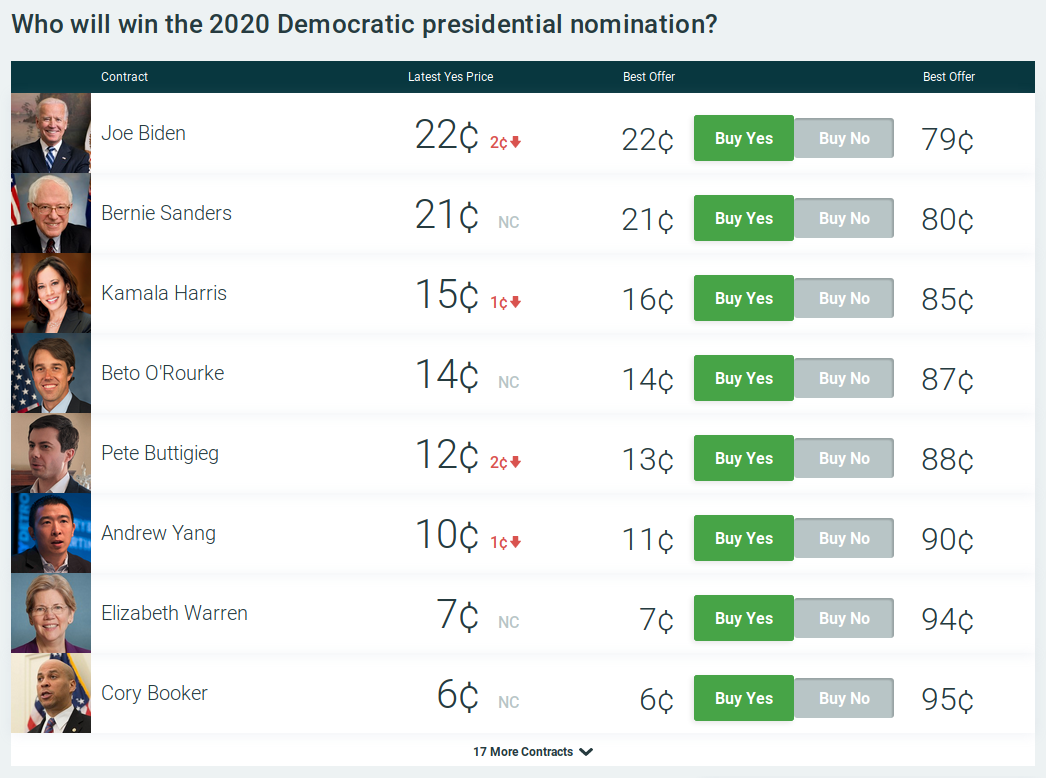
\includegraphics{2020_dem_primary.png}
\caption{Democratic Primary Market}
\end{figure}

\end{frame}

\begin{frame}{PredicIt Data}
\protect\hypertarget{predicit-data}{}

\begin{longtable}[]{@{}lllrr@{}}
\caption{Market Data (44,711 observations with 6 of 11
variables)}\tabularnewline
\toprule
ID & Ticker & Date & Price & Volume\tabularnewline
\midrule
\endfirsthead
\toprule
ID & Ticker & Date & Price & Volume\tabularnewline
\midrule
\endhead
3484 & MCCA.MOSENATE.2018 & 2017-09-20 & 0.47 & 0\tabularnewline
2940 & SANDERS.VTSENATE.2018 & 2017-11-06 & 0.86 & 0\tabularnewline
3532 & LEWI.MN02.2018 & 2018-06-08 & 0.40 & 0\tabularnewline
3608 & HELL.NVSENATE.2018 & 2018-07-17 & 0.33 & 101\tabularnewline
4232 & CASE.PASENATE.2018 & 2018-07-18 & 0.89 & 0\tabularnewline
3767 & NH01.2018 & 2018-08-06 & 0.82 & 0\tabularnewline
3736 & PA15.2018 & 2018-08-24 & 0.95 & 26\tabularnewline
4258 & NJ07.2018 & 2018-09-03 & 0.41 & 2\tabularnewline
2918 & WARREN.MASENATE.2018 & 2018-10-23 & 0.96 & 1354\tabularnewline
4304 & WI01.2018 & 2018-11-07 & 0.99 & 1019\tabularnewline
\bottomrule
\end{longtable}

\end{frame}

\begin{frame}{Messy Data}
\protect\hypertarget{messy-data}{}

\begin{longtable}[]{@{}llrr@{}}
\caption{Messy Combined (9,200 observations of 4
variables)}\tabularnewline
\toprule
Date & Race & Market Price & Model Probability\tabularnewline
\midrule
\endfirsthead
\toprule
Date & Race & Market Price & Model Probability\tabularnewline
\midrule
\endhead
2018-08-01 & AZ-S1 & 0.66 & 0.738\tabularnewline
2018-08-01 & CA-10 & 0.58 & 0.705\tabularnewline
2018-08-01 & CA-12 & 0.91 & 1.000\tabularnewline
2018-08-01 & CA-22 & 0.30 & 0.049\tabularnewline
2018-08-01 & CA-25 & 0.61 & 0.745\tabularnewline
2018-08-01 & CA-39 & 0.61 & 0.377\tabularnewline
2018-08-01 & CA-48 & 0.72 & 0.666\tabularnewline
2018-08-01 & CA-49 & 0.74 & 0.795\tabularnewline
2018-08-01 & CA-S1 & 0.94 & 1.000\tabularnewline
2018-08-01 & CO-05 & 0.06 & 0.027\tabularnewline
\bottomrule
\end{longtable}

\end{frame}

\begin{frame}{Tidy Data}
\protect\hypertarget{tidy-data}{}

\begin{longtable}[]{@{}lllr@{}}
\caption{Tidy Combined (18,400 observations of 4
variables)}\tabularnewline
\toprule
Date & Race & Predictive Method & Probability\tabularnewline
\midrule
\endfirsthead
\toprule
Date & Race & Predictive Method & Probability\tabularnewline
\midrule
\endhead
2018-08-01 & AZ-S1 & market & 0.660\tabularnewline
2018-08-01 & AZ-S1 & model & 0.738\tabularnewline
2018-08-01 & CA-10 & market & 0.580\tabularnewline
2018-08-01 & CA-10 & model & 0.705\tabularnewline
2018-08-01 & CA-12 & market & 0.910\tabularnewline
2018-08-01 & CA-12 & model & 1.000\tabularnewline
2018-08-01 & CA-22 & market & 0.300\tabularnewline
2018-08-01 & CA-22 & model & 0.049\tabularnewline
2018-08-01 & CA-25 & market & 0.610\tabularnewline
2018-08-01 & CA-25 & model & 0.745\tabularnewline
\bottomrule
\end{longtable}

\end{frame}

\begin{frame}{Race Distributions}
\protect\hypertarget{race-distributions}{}

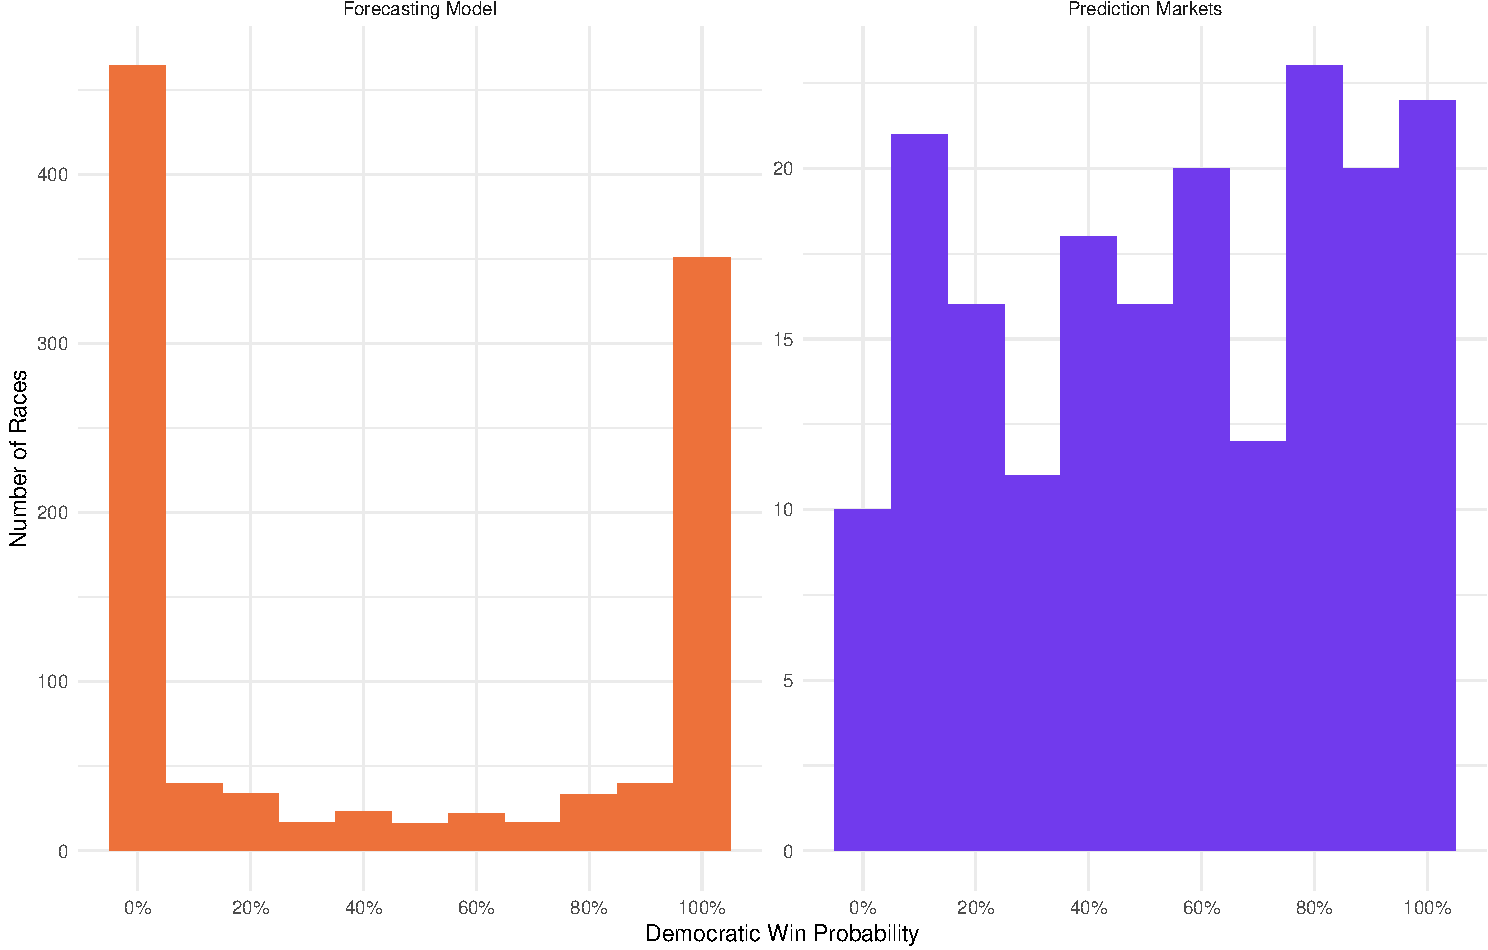
\includegraphics{presentation_files/figure-beamer/plot_races_hist-1.pdf}

\end{frame}

\begin{frame}{Method Similarities}
\protect\hypertarget{method-similarities}{}

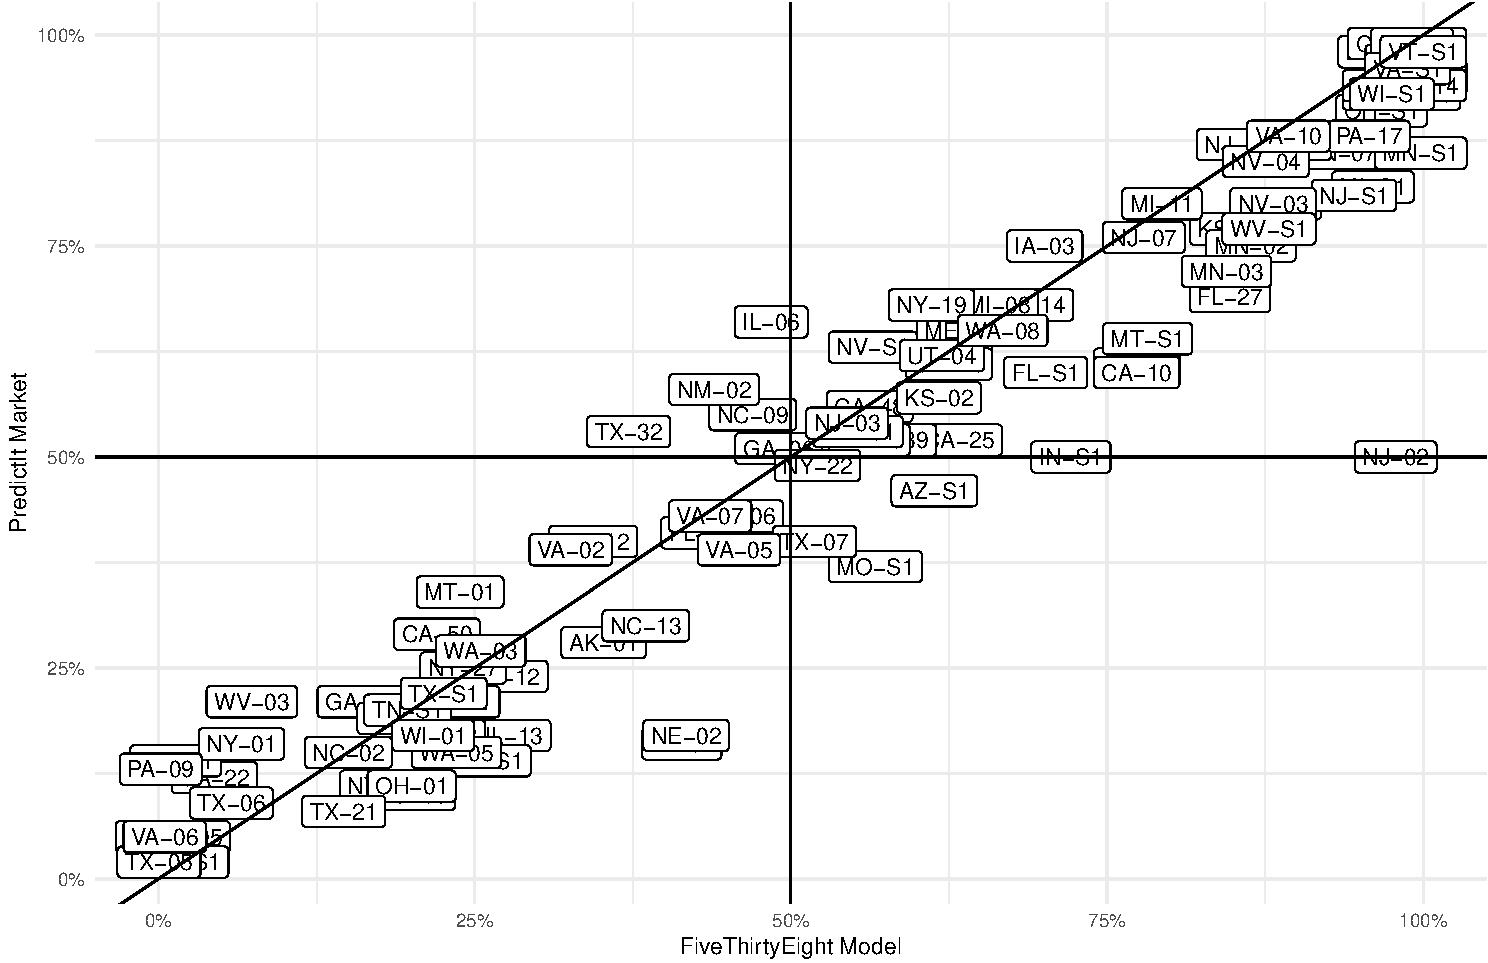
\includegraphics{presentation_files/figure-beamer/plot_cartesian_races-1.pdf}

\end{frame}

\begin{frame}{Market Manipulation?}
\protect\hypertarget{market-manipulation}{}

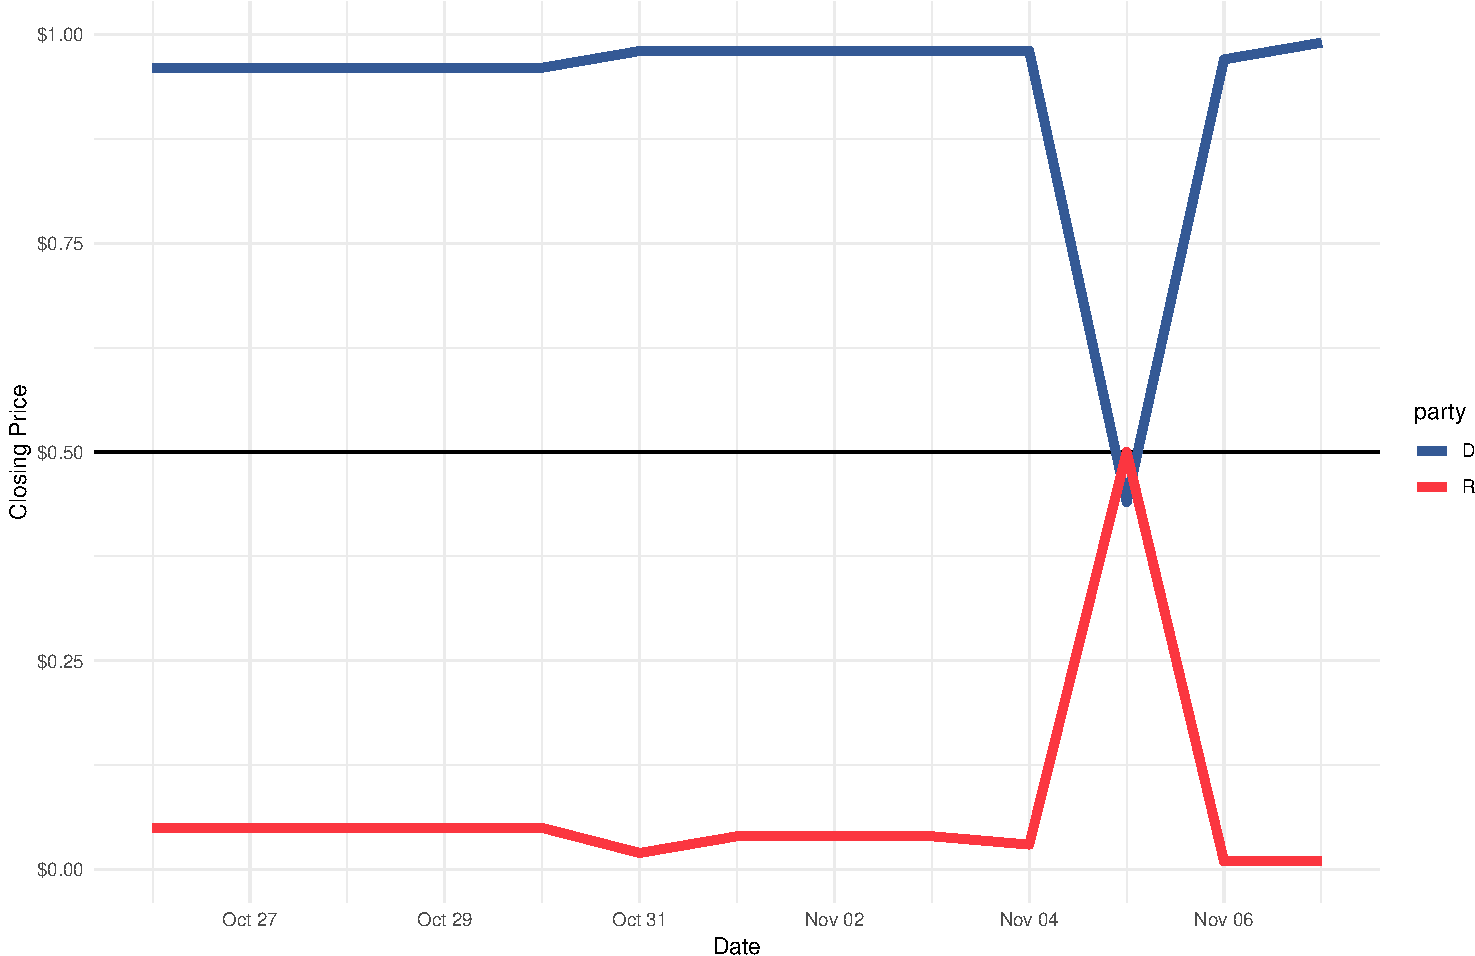
\includegraphics{presentation_files/figure-beamer/plot_nj_02-1.pdf}

\end{frame}

\begin{frame}{Method Accuracy}
\protect\hypertarget{method-accuracy}{}

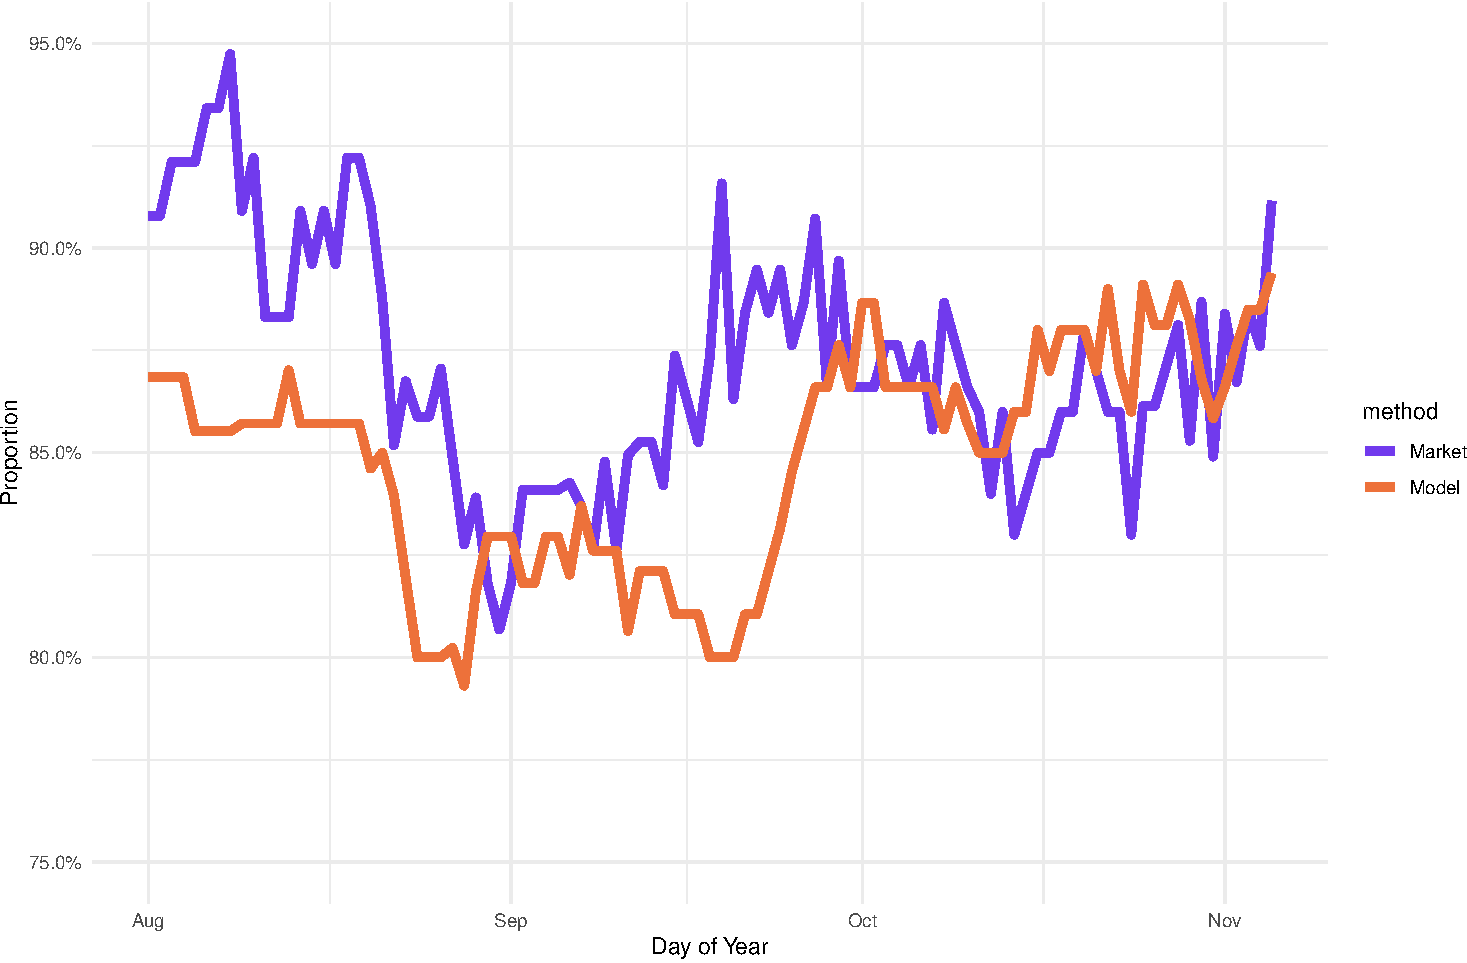
\includegraphics{presentation_files/figure-beamer/prop_day_line-1.pdf}

\end{frame}

\begin{frame}{Method Accuracy}
\protect\hypertarget{method-accuracy-1}{}

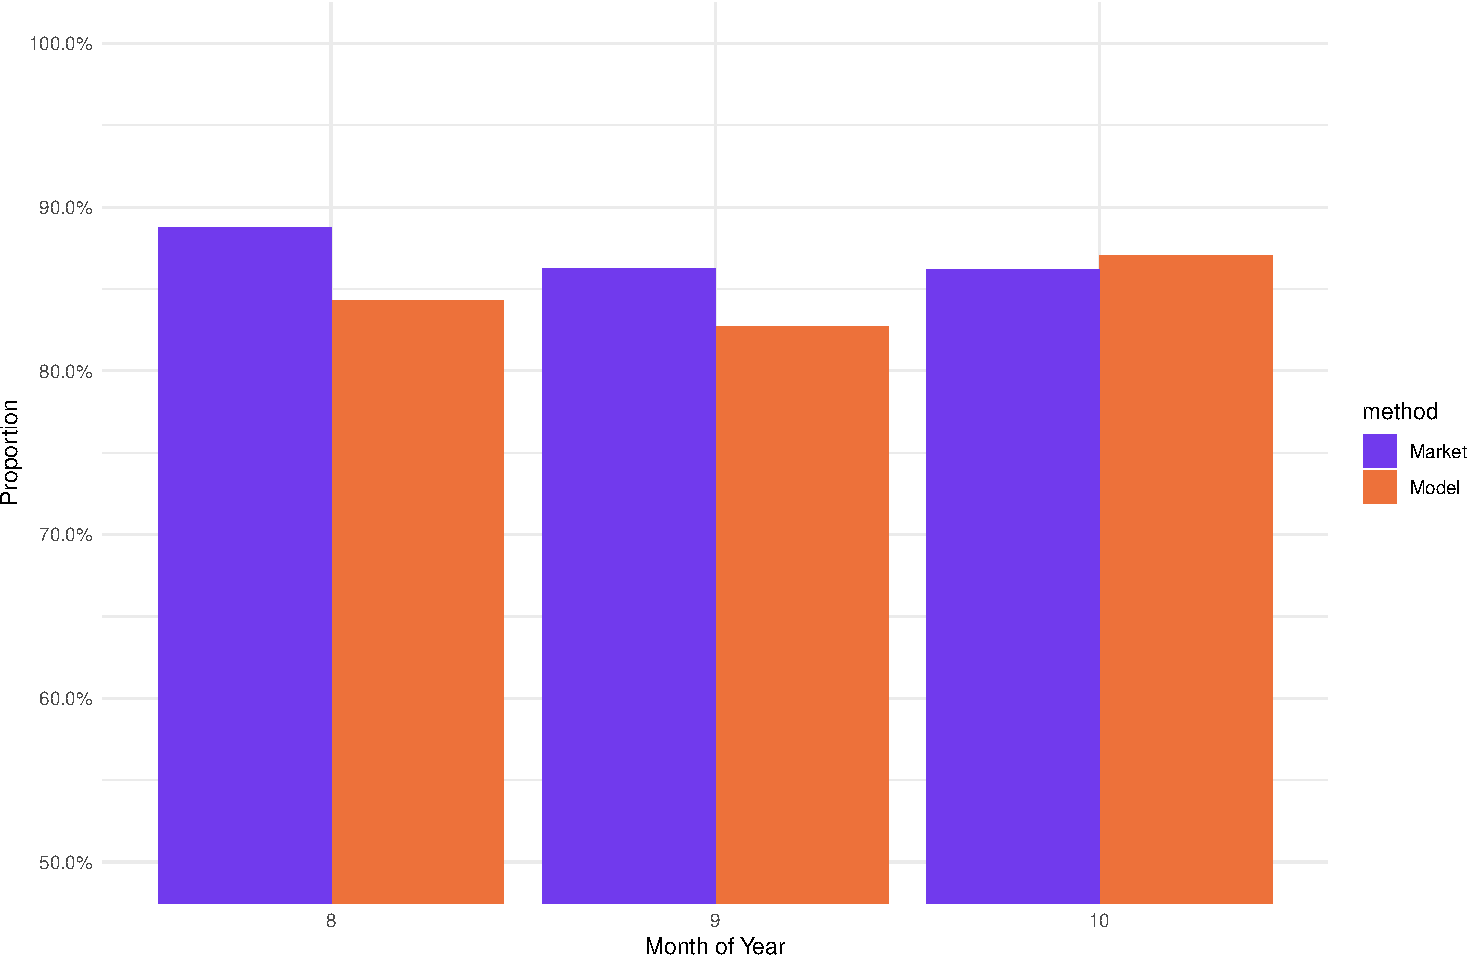
\includegraphics{presentation_files/figure-beamer/prop_month_bars-1.pdf}

\end{frame}

\end{document}
